%!TEX root = ../template.tex
%%%%%%%%%%%%%%%%%%%%%%%%%%%%%%%%%%%%%%%%%%%%%%%%%%%%%%%%%%%%%%%%%%%
%% chapter3.tex
%% UNIPD thesis document file
%%
%% Chapter with introduction
%%%%%%%%%%%%%%%%%%%%%%%%%%%%%%%%%%%%%%%%%%%%%%%%%%%%%%%%%%%%%%%%%%%

\typeout{NT FILE chapter3.tex}%

\chapter{Fondamenti Teorici}

\prependtographicspath{{Chapters/Figures/Covers/}}

\section{Sistemi embedded e IoT}

\subsection{Introduzione ai sistemi embedded}
\noindent

I sistemi embedded sono sistemi di elaborazione integrati all'interno dell'oggetto o del sistema informatico, progettati per compiti specifici, che offrono un'elevata efficienza e un basso consumo energetico rispetto ai sistemi general-purpose. Sono sempre più utilizzati in applicazioni come l'elaborazione audio e i sistemi di controllo in tempo reale in vari ambienti, tra cui l'industria della ristorazione. Grazie alla loro flessibilità, questi sistemi possono integrarsi perfettamente in ambienti complessi dove l'affidabilità e la compattezza sono fattori critici.

Nel contesto dei sistemi audio per ristoranti, le piattaforme embedded come Raspberry Pi sono ideali per gestire flussi audio in tempo reale, decodificare l'audio digitale e garantire uscite audio sincronizzate per le diverse zone di un ristorante, come i singoli tavoli.

La loro scalabilità ed economicità le rendono adatte a implementare ambienti audio personalizzati in locali di medie e grandi dimensioni.


\subsection{L'IoT in ambito ristorativo}
\noindent

L'\gls{iot} ha rivoluzionato il settore della ristorazione, consentendo ai dispositivi di interagire e scambiare dati in modo autonomo. Nei ristoranti intelligenti, i dispositivi \gls{iot} possono gestire tutto, dal servizio clienti al controllo dell'ambiente. Una delle applicazioni più innovative è l'uso dell'\gls{iot} per creare ambienti sonori personalizzati, o “bolle sonore”, dove ogni tavolo può avere il proprio percorso sonoro su misura.

L'integrazione di sensori e dispositivi audio consente ai ristoranti di monitorare e regolare in tempo reale i livelli audio, il rumore ambientale e le preferenze dei clienti. Ad esempio, la musica di sottofondo può essere regolata automaticamente in base ai dati in tempo reale, come il feedback dei clienti o i livelli di rumore.

Le tecnologie \gls{iot} in questo contesto offrono un'esperienza utente più fluida , aumentando la soddisfazione dei clienti e l'efficienza operativa.

L'implementazione di queste tecnologie non si limita a migliorare l'esperienza audio nei ristoranti ma contribuisce anche a migliorare la sicurezza. I sensori  possono essere applicati per monitorare l'ambiente della cucina e inviare avvisi in caso di pericolo di incendio o possono monitorare le operazioni di cucina, rendendo il ristorante più reattivo ed efficiente.

\subsection{Raspberry Pi come piattaforma per sistemi audio}
\noindent

Il Raspberry Pi è ampiamente riconosciuto come piattaforma ideale per i sistemi embedded nelle applicazioni audio, grazie al suo basso costo, alla versatilità e alla sufficiente potenza di elaborazione.

In questo progetto di tesi, il Raspberry Pi Zero 2W viene utilizzato come unità di elaborazione centrale per gestire i flussi audio e distribuirli ai singoli dispositivi sul tavolo. Il sistema sfrutta Mopidy, un server di streaming basato su Python, insieme a Iris per i controlli frontend, consentendo la gestione in tempo reale di playlist e livelli audio. L'integrazione del Pi con \gls{dac} e \gls{gpio} consente inoltre di formare un'architettura di sistema flessibile che può essere ampliata con sensori o interfacce audio aggiuntive.

Il supporto di Raspberry Pi per il multitasking e la sua capacità di gestire l'elaborazione in parallelo lo rendono uno dei migliori candidati per le attività di elaborazione audio in un ristorante, dove è necessario gestire in modo efficiente più canali.

Inoltre, la compatibilità di questo dispositivo con varie librerie software,  consente al sistema di essere altamente personalizzabile e adattabile a diversi ambienti.

\section{Tecnologie di streaming audio}

\subsection{Panoramica delle tecnologie di streaming audio}
\noindent

Lo streaming audio si riferisce alla trasmissione in tempo reale di dati audio su una rete, consentendo agli utenti di ascoltare l'audio senza doverlo scaricare in locale. Questa tecnologia si basa su protocolli che gestiscono il flusso costante di pacchetti di dati tra server e client  per garantire una riproduzione fluida. Due dei protocolli più utilizzati sono il \gls{rtsp} e l'\gls{hls}.

\begin{itemize}
    \item \gls{rtsp} stabilisce e controlla uno o più flussi sincronizzati nel 
          tempo di media continui, come audio. In genere non fornisce 
          direttamente i flussi continui, anche se è possibile l'interleaving del 
          flusso multimediale continuo con il flusso di controllo. In altre parole, 
          \gls{rtsp} agisce come un ``telecomando di rete'' per i server 
          multimediali.
          
    \item \gls{hls}, è un formato adattativo basato su \gls{http} per il trasporto 
          di dati video e audio dai server multimediali agli schermi degli 
          spettatori. I contenuti video e audio vengono suddivisi in una serie di 
          pezzi, compressi per una consegna rapida e trasmessi ai dispositivi 
          degli utenti finali. Gli spettatori godono quindi di uno streaming fluido, 
          nonostante tutto ciò che accade in background. La popolarità di 
          questo protocollo rispetto alle sue alternative è dovuta alla 
          compatibilità della riproduzione e alla qualità dell'esperienza. Infatti, 
          tutti i dispositivi Mac, Android, Microsoft e Linux sono in grado di 
          riprodurre flussi trasmessi con \gls{hls}.
  \end{itemize}

Entrambi i protocolli sono essenziali per mantenere una trasmissione audio a bassa latenza e di alta qualità, particolarmente importante in scenari che richiedono la sincronizzazione di più flussi in zone diverse.

\subsection{Mopidy: Architettura e caratteristiche}
\noindent

Mopidy è un servizio open-source  basato su Python, progettato per gestire e riprodurre audio sia in locale che online. Funziona come un server \gls{http}, consentendo agli utenti di controllare la musica attraverso interfacce web e altri dispositivi remoti. Mopidy viene spesso utilizzato in ambienti in cui è richiesto lo streaming audio multi-room, offrendo una soluzione flessibile e personalizzabile per spazi pubblici e privati. Questo sistema supporta diverse interfacce frontend, come Iris, e può integrarsi con piattaforme come Spotify, SoundCloud, e file system locali.

Uno dei punti di forza di Mopidy è la sua architettura modulare, che consente agli sviluppatori di estendere le sue capacità attraverso un'ampia gamma di plugin. Questa modularità rende Mopidy altamente adattabile a diverse applicazioni, dalle configurazioni audio domestiche agli ambienti commerciali in cui l'audio deve essere trasmesso in più zone.

L'uso dell'architettura client-server di Mopidy è particolarmente adatto alla gestione di più flussi audio in rete. Ogni client può essere collegato a una serie di altoparlanti, mentre il server gestisce la riproduzione del file audio. Mopidy spesso è abbinato a Snapcast, un altro strumento che sincronizza l'audio tra più client. Snapcast assicura che tutti i client rimangano sincronizzati, riproducendo lo stesso flusso audio senza ritardi evidenti. Questo sistema consente un controllo preciso sulla riproduzione audio in più luoghi, rendendolo ideale per spazi pubblici come scuole, uffici o campus di più edifici.

Il server Mopidy può essere controllato da remoto utilizzando una varietà di interfacce, consentendo agli utenti di gestire playlist, controllare il volume e programmare la riproduzione utilizzando interfacce basate sul web e a riga di comando. Questa flessibilità rende Mopidy una soluzione molto efficace per gli ambienti in cui l'audio deve essere gestito da una postazione centrale.~\cite{cit-mopidy}

\section{Acustica nei ristoranti}

\subsection{L'importanza dell'ambiente acustico nei ristoranti}
\noindent

Uno degli elementi chiave che definiscono la qualità acustica di uno spazio è il \gls{rt60}, che misura il tempo necessario del suono per dissolversi in un determinato ambiente. Nei ristoranti, ad esempio, un riverbero elevato può compromettere la chiarezza di un discorso, costringendo i clienti ad alzare la voce, con conseguente aumento dei livelli di rumore. Di conseguenza, un tempo di riverberazione ben controllato consente una comunicazione più chiara, creando un ambiente più confortevole per il cliente.

Allo stesso modo, l'equilibrio tra assorbimento e riflessione del suono gioca un ruolo cruciale nel determinare il comfort acustico complessivo. Materiali come pannelli acustici, tappeti e imbottiture possono essere posizionati strategicamente per ridurre la riflessione delle onde sonore. Quando le superfici sono molto riflettenti, creano echi e sovrapposizioni di onde sonore, che possono rendere l'ambiente caotico e sgradevole.

L'acustica e il comportamento umano sono correlati. Alti livelli di rumore nei ristoranti sono spesso associati a un aumento dello stress, a una riduzione del comfort e persino a una percezione negativa del cibo e del servizio. Alcuni studi hanno dimostrato che gli ambienti rumorosi possono portare a soggiorni più brevi e a un consumo più rapido dei pasti, in quanto i clienti possono trovare difficile rilassarsi.

Inoltre, è dimostrato che il suono può influenzare la percezione del gusto (Cap 4). Le ricerche suggeriscono che livelli di rumore più bassi consentono ai clienti di concentrarsi maggiormente sulle sottigliezze del gusto e della consistenza, migliorando l'esperienza gastronomica complessiva. Al contrario, ambienti rumorosi e caotici possono offuscare queste percezioni, portando a un'esperienza meno piacevole.

Trovare il giusto equilibrio tra garantire il comfort acustico e creare un'atmosfera vivace è una delle sfide principali dell'acustica dei ristoranti. Molti locali moderni privilegiano spazi aperti, superfici dure e soffitti alti che, pur essendo esteticamente gradevoli, tendono ad amplificare il suono e ad esacerbare i livelli di rumore. Queste scelte progettuali possono determinare un ambiente acusticamente svantaggioso, soprattutto se combinato con un'alta densità di clienti.

Per mitigare questi problemi, i designer devono incorporare trattamenti acustici che non compromettano l'estetica dello spazio. Soluzioni come pannelli radianti a soffitto, pareti rivestite in tessuto e arredamento fonoassorbente possono contribuire a creare uno spazio in grado di bilanciare l'atmosfera con la chiarezza acustica.~\cite{wiki:sound-restaurants}

\subsection{Il concetto di Bolle Sonore}
\noindent

Il concetto di "bolle sonore ” si riferisce alla creazione di microambienti acustici personalizzati all'interno di uno spazio condiviso più ampio. In pratica, si tratta di progettare una configurazione audio in cui zone o aree diverse, come i singoli tavoli di un ristorante, possono avere paesaggi sonori isolati o personalizzati senza interferenze dai flussi audio circostanti. Le bolle sonore mirano a fornire un'esperienza uditiva mirata e coinvolgente per ogni ascoltatore o gruppo, migliorando la privacy e riducendo gli effetti negativi del rumore di fondo.

La creazione di bolle sonore richiede un preciso isolamento acustico e il controllo della distribuzione del suono. Questo può essere ottenuto attraverso una combinazione di barriere fisiche, altoparlanti direzionali e tecnologie di cancellazione del suono. I diffusori direzionali, ad esempio, concentrano i fasci audio in direzioni specifiche, impedendo al suono di diffondersi in altre aree. Allo stesso modo, i pannelli acustici o i divisori possono aiutare a bloccare le onde sonore dal passaggio oltre le zone designate.

In molti casi, la tecnologia utilizzata per creare bolle sonore coinvolge sistemi audio multi-room. Questi sistemi consentono di trasmettere flussi audio diversi alle varie parti di uno spazio, permettendo a ogni zona di avere un ambiente sonoro indipendente. Il sistema garantisce che ogni zona riceva il contenuto audio desiderato senza interferenze dalle zone adiacenti.

Snapcast, ad esempio, è un software molto diffuso che consente lo streaming audio sincronizzato su più dispositivi. Garantisce che tutti i client audio riproducano lo stesso flusso senza ritardi, rendendolo ideale per gli ambienti in cui la tempistica e il coordinamento sono fondamentali. In combinazione con Mopidy, che funge da server audio, Snapcast può trasmettere flussi audio distinti ad aree separate, creando bolle sonore controllate.

Oltre alle soluzioni basate sul software, l'hardware, come gli altoparlanti direzionali, può focalizzare il suono in direzioni specifiche, assicurando che solo il pubblico previsto lo senta chiaramente. Questi diffusori possono essere posizionati sopra o intorno a un'area specifica, ad esempio un tavolo da pranzo, per proiettare il suono direttamente nell'area di destinazione, riducendo al minimo la diffusione nelle zone adiacenti. Questa tecnologia è particolarmente utile negli ambienti open space, dove la gestione della dispersione sonora tra le zone è fondamentale.

Nelle applicazioni pratiche, le bolle sonore vengono utilizzate per creare ambienti audio personalizzati in spazi pubblici condivisi. Ad esempio, in un ristorante, ogni tavolo può avere un'esperienza sonora personalizzata, che si tratti di musica, conversazioni o altri contenuti audio. In questo modo i clienti possono godere di un'esperienza sonora più intima e controllata, senza la distrazione di conversazioni vicine o rumori di fondo. 

Oltre che nei ristoranti, le bolle sonore trovano applicazione in vari spazi commerciali e pubblici, come musei, uffici e biblioteche, dove il controllo dell'ambiente uditivo è essenziale per migliorare l'esperienza degli utenti. Questi ambienti traggono vantaggio in quanto aiutano a bilanciare privacy, concentrazione e atmosfera senza ricorrere a un isolamento acustico completo.~\cite{cit-multiaudio}

\section{Reti neurali artificiali per la previsione del gradimento alimentare}

\subsection{Introduzione alle reti neurali artificiali nel contesto della previsione del gradimento alimentare}
\noindent

Nei paragrafi è stato dimostrato che le caratteristiche acustiche, come il livello e il tipo di rumore [8-14] e i fattori non acustici, come l'età, il sesso e la sensibilità al rumore, possono influenzare il gradimento del cibo in presenza di rumore di fondo. Tuttavia, il contributo relativo dei fattori acustici e non acustici al gradimento del cibo in presenza di rumore di fondo è ancora sconosciuto.

Le \gls{ann} sono state utilizzate in molte applicazioni negli ultimi vent'anni per la classificazione (e.g. addestramento per classificare le immagini in "cani" o "gatti" ), il riconoscimento di pattern (e.g. il riconoscimento facciale), la regressione e la previsione (e.g. la previsione del flusso di un fiume) \cite{rezaeianzadeh2014flood}.

Esse rappresentano un potente strumento di apprendimento automatico ispirato al funzionamento del cervello umano. 

I principali vantaggi delle \gls{ann} nella previsione del gradimento alimentare includono:

\begin{itemize}
    \item \textbf{Modellazione di relazioni non lineari}: Possiedono una notevole capacità di catturare e modellare relazioni non lineari complesse tra variabili di input e output, senza richiedere assunzioni preliminari sulla forma di queste relazioni. Questa caratteristica è particolarmente preziosa quando si tratta di modellare fenomeni complessi come le preferenze alimentari.
    \item \textbf{Gestione di dati multidimensionali}: La  capacità di processare efficacemente dati multidimensionali ed elaborare simultaneamente molteplici variabili di input, che nel contesto dell'analisi del gradimento alimentare possono includere fattori acustici, caratteristiche individuali e parametri ambientali.
    \item \textbf{Apprendimento adattivo}: Le \gls{ann} possono aggiornare continuamente i loro parametri con l'introduzione di nuovi dati, migliorando costantemente le prestazioni predittive nel tempo. Questo le rende strumenti particolarmente flessibili e adattabili a diversi contesti applicativi.
    \item \textbf{Robustezza al rumore nei dati}: Robustezza nell'elaborazione di dati rumorosi o incompleti, caratteristica particolarmente preziosa quando si lavora con valutazioni soggettive umane, dove la variabilità naturale delle risposte e l'influenza di fattori esterni non controllabili sono intrinseche al processo di raccolta dati.
\end{itemize}

Le \gls{ann} hanno dimostrato la loro efficacia in diversi ambiti della valutazione alimentare, come la previsione delle valutazioni dell'appetito. Tuttavia, prima dello studio presentato in \cite{alamir2021enhanced}, non erano mai state applicate alla previsione dell'apprezzamento del cibo in presenza di rumore di fondo, nonostante la loro comprovata superiorità rispetto ai modelli statistici tradizionali nel gestire relazioni non lineari. Questa caratteristica è particolarmente rilevante nel contesto dell'esperienza gastronomica, dove la relazione tra stimoli acustici e percezione del gusto presenta evidenti non linearità che i modelli statistici classici faticano a catturare.

L'utilizzo delle \gls{ann} in questo campo apre nuove frontiere per comprendere e prevedere come diversi fattori ambientali, in particolare il rumore, influenzano l'esperienza gastronomica. Questa comprensione non solo ha implicazioni pratiche per l'industria della ristorazione, ma offre anche preziosi spunti sulle complesse interazioni tra i nostri sensi nella percezione del cibo. La ricerca proposta mira a esplorare e quantificare queste interazioni attraverso l'implementazione di un modello \gls{ann} avanzato, con l'obiettivo di fornire uno strumento predittivo accurato e versatile per l'ottimizzazione dell'esperienza culinaria in diversi ambienti acustici.

\subsection{Architettura delle ANN}
\noindent

Le \gls{ann} si basano su un'architettura \gls{mlp} progettata per predire il gradimento del cibo in presenza di rumori di sottofondo. La struttura è stata attentamente organizzata in tre componenti principali che lavorano in sinergia per elaborare e analizzare i dati.

La struttura della rete è così articolata:

\begin{itemize}
    \item \textbf{Strato di input}: che funge da porta d'ingresso per i dati. Questo strato comprende cinque neuroni, ognuno dedicato a un fattore specifico:
    \begin{enumerate}
        \item Età
        \item Genere
        \item Sensibilità al rumore
        \item Tipo di rumore
        \item Livello di rumore
    \end{enumerate}

    Questi elementi rappresentano le variabili fondamentali che influenzano la percezione del cibo in un ambiente rumoroso.
    
    \item \textbf{Strati nascosti}: Due strati nascosti, ognuno contenente dieci neuroni. Questi strati sono cruciali per l'elaborazione dei dati, in quanto utilizzano una funzione di attivazione non lineare \gls{tanh} per processare le informazioni. Le connessioni tra i neuroni sono unidirezionali, con pesi che possono variare tra -1 e 1, permettendo alla rete di modulare l'importanza relativa di ogni connessione.
    
    \item \textbf{Strato di output}: Elabora tutte queste informazioni attraverso una funzione di attivazione lineare per produrre il risultato finale: una valutazione che indica quanto il cibo viene apprezzato nelle diverse condizioni sonore.
\end{itemize}

\begin{figure}[H]
      \centering
      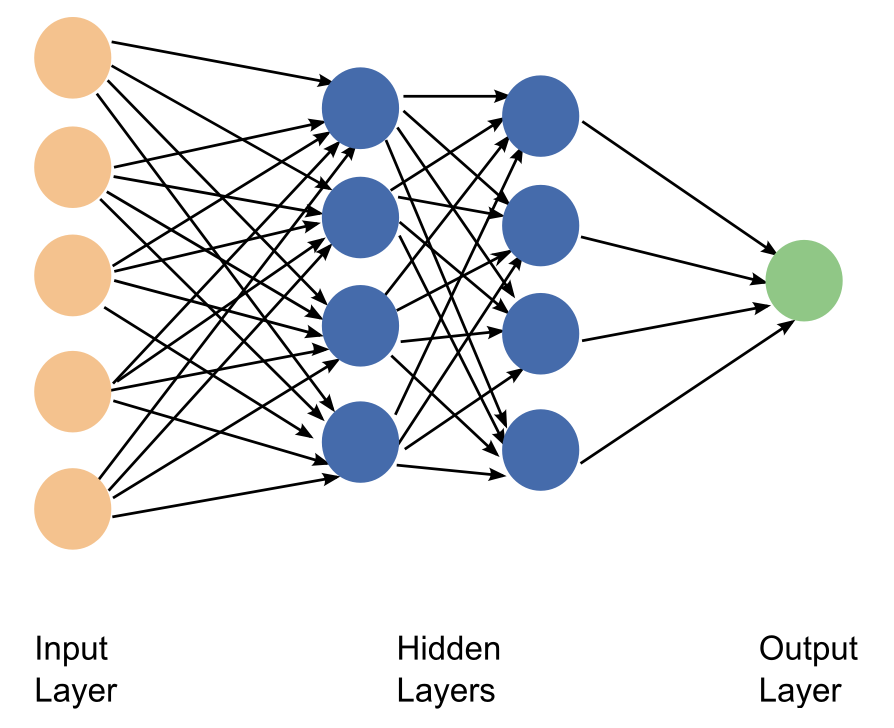
\includegraphics[width=0.6\textwidth]{Chapters/Figures/ArchitectureANN.png}
      \caption{\small Architettura delle reti neurali. Lo strato di ingresso contiene fattori predittivi, mentre lo strato di uscita contiene le valutazioni di gradimento dei cibi. Gli strati sovrapposti o gli strati nascosti hanno un certo numero di neuroni.}
      \label{fig:architectureann}
  \end{figure}

  L'output di ciascuno layer l è dato dalla formula:

\begin{equation}
  O_i^{(l)} = \varphi(u_i^{(l)}) = \varphi(\sum_{j=1}^{nl} O_j^{(l-1)} w_{ji}^{(l)} + w_{0,i}^{(l)}), 1 \le l \le L
\end{equation}
  dove $u$ è la funzione di attivazione (solitamente una funzione \gls{tanh} non lineare per gli strati nascosti e una funzione lineare per lo strato di output), $l$ è l'indice dello strato, $w_{j,i}^{(l)}$ sono i pesi delle interconnessioni tra i neuroni, e $w_{0,i}^{(l)}$ sono i bias dei neuroni.

  Questa architettura \gls{mlp} con connessioni bidirezionali tra gli strati è stata utilizzata per modellare la complessità delle relazioni tra i fattori di ingresso e la gradevolezza relativa del cibo.

\begin{comment}
La scelta di questa architettura è stata motivata da una serie di considerazioni:

\begin{itemize}
    \item \textbf{Complessità del problema}: I due strati nascosti permettono alla rete di catturare relazioni non lineari complesse tra gli input e l'output.
    
    \item \textbf{Bilanciamento tra complessità e generalizzazione}: Il numero di neuroni negli strati nascosti (10 per strato) è stato selezionato per fornire sufficiente capacità di modellazione senza rischiare il fenomeno dell'overfitting.
    
    \item \textbf{Funzioni di attivazione}: La funzione \texttt{tanh} negli strati nascosti introduce non linearità, mentre la funzione lineare nello strato di output consente previsioni continue del gradimento.
    
    \item \textbf{Input multidimensionali}: Lo strato di input con 5 neuroni permette l'integrazione di fattori sia acustici che non acustici, riflettendo la natura multidimensionale del problema.
\end{itemize}

Questa architettura consente alla rete di processare efficacemente l'interazione tra fattori demografici (età, genere), individuali (sensibilità al rumore) e ambientali (tipo e livello di rumore) nella determinazione del gradimento alimentare. La capacità della rete di modellare queste interazioni complesse la rende particolarmente adatta per questo tipo di previsione, superando le limitazioni dei modelli lineari tradizionali.

L'efficacia di questa architettura sarà ulteriormente potenziata dall'applicazione dell'algoritmo di ottimizzazione Harris Hawks, che verrà discusso nella sezione successiva.
\end{comment}

\subsection{L'algoritmo di ottimizzazione Harris Hawks Optimization (HHO)}
\noindent

L'algoritmo \gls{hho} è una tecnica di ottimizzazione meta-euristica ispirata alla natura, che migliora significativamente le prestazioni delle \gls{ann} nella previsione del gradimento dei cibi. 

L'\gls{hho} imita il comportamento dei falchi Harris durante la cattura delle lepri, rappresentando la fase di ottimizzazione globale o di esplorazione ed sfruttamento, cioè:

\begin{itemize}
      \item \textbf{Esplorazione}: In questa fase, l'algoritmo \gls{hho} cerca di esplorare nuove regioni dello spazio di ricerca, al fine di trovare soluzioni promettenti che potrebbero non essere state ancora scoperte. Questo viene fatto attraverso l'utilizzo di una strategia di ricerca casuale, come l'equazione (3.2) presentata nel documento, che permette di aggiornare la soluzione corrente ($X(t)$) verso soluzioni casuali ($X_r(t)$).

      L'obiettivo dell'esplorazione è quello di evitare il rischio di rimanere bloccati in ottimi locali, ampliando la ricerca per trovare potenziali soluzioni migliori.

      \item \textbf{Sfruttamento}: Nella fase di sfruttamento, l'algoritmo \gls{hho} cerca di migliorare e affinare le migliori soluzioni trovate finora, allo scopo di convergere verso l'ottimo globale. Questo viene fatto attraverso l'aggiornamento della soluzione corrente ($X(t)$) verso la migliore soluzione trovata finora ($x_b(t)$), come mostrato nell'equazione (4).
      
      Lo sfruttamento permette di concentrare la ricerca sulle regioni più promettenti dello spazio di ricerca, sfruttando le conoscenze acquisite nelle precedenti iterazioni. 

\end{itemize}

L'alternanza tra esplorazione e sfruttamento è cruciale per l'efficacia degli algoritmi metauristici come l'\gls{hho}, in quanto permette di bilanciare la capacità di esplorare nuove soluzioni e quella di sfruttare le migliori soluzioni trovate finora, al fine di convergere rapidamente verso l'ottimo globale.

Nella fase iniziale, l'algoritmo \gls{hho} genera casualmente un set di $N$ soluzioni candidate, che vengono rappresentate come il vettore $X$. Queste soluzioni candidate rappresentano i possibili punti all'interno dello spazio di ricerca in cui si sta cercando di trovare la soluzione ottimale.

Una volta generato questo set iniziale di soluzioni, l'\gls{hho} procede a calcolare la funzione di fitness per ciascuna di queste soluzioni candidate. La funzione di fitness è una misura quantitativa di quanto una data soluzione sia "buona" o "vicina" all'ottimo che si sta cercando.

Tipicamente, la funzione di fitness viene definita in modo tale che le soluzioni migliori (cioè quelle più vicine all'ottimo) abbiano un valore di fitness più elevato rispetto alle soluzioni peggiori. Questo permette all'algoritmo di identificare la migliore soluzione trovata finora, che viene denominata "posizione della lepre" ($x_b$).

Successivamente, durante la fase di esplorazione e sfruttamento, l'\gls{hho} utilizza le equazioni (3.2) e (3.3) per aggiornare iterativamente le soluzioni candidate ($X$), alternando tra la ricerca di nuove soluzioni promettenti (esplorazione) e il miglioramento delle migliori soluzioni trovate finora (sfruttamento). 

Questo processo iterativo continua finché non viene soddisfatto un criterio di arresto, ad esempio un numero massimo di iterazioni o il raggiungimento di una soglia di fitness desiderata.

La rappresentazione matematica dell'algoritmo HHO è espressa come:

\begin{equation}
      X(t+1) =
      \begin{cases}
            X_r(t) - r_1 |X_r(t) - 2r_2 X(t)| &  q \ge 0.5 \\
            X_b(t) - X_m(t) - r_3 (lb + r_4 (ub - lb)) & \text{otherwise}
      \end{cases}
\end{equation} 

Dove $X_r(t)$  è una soluzione casuale selezionata dal pool di soluzioni candidate, $X_{b}(t)$ è la migliore soluzione trovata finora, $X_{m}(t)$ è la soluzione media, $r_1$, $r_2$, $r_3$, $r_4$ sono numeri casuali, $q$ è un numero casuale compreso tra 0 e 1 che determina la probabilità di passare tra due stati, e $lb$ e $ub$ sono i limiti inferiore e superiore dello spazio di ricerca.

Quando $q\geq0.5$ l'\gls{hho} segue la fase di esplorazione. Altrimenti, l'algoritmo passa alla fase di sfruttamento, utilizzando l'equazione:

\begin{equation}
      X(t+1) = \Delta X(t) - E|J \times X_b(t) - X(t)| 
\end{equation}

Dove $\Delta X(t)$ è la differenza tra $X_{b}(t)$ e $X(t)$, e $J = 2(1-r_{5})$ rappresenta i salti casuali della lepre, con r5 un numero casuale tra 0 e 1.

Semplificando:

\begin{equation}
      X(t+1) = X_{b}(t) - E|\Delta X(t)|
\end{equation}

\begin{comment}

\textbf{Implementazione nell'ottimizzazione delle RNA:}

Nel nostro studio, l'HHO viene impiegato per ottimizzare i pesi e le polarizzazioni della RNA, sostituendo i tradizionali metodi di retropropagazione. Questo approccio offre diversi vantaggi:

\begin{itemize}
    \item \textbf{Ottimizzazione globale}: La capacità dell'HHO di esplorare l'intero spazio delle soluzioni aiuta a evitare gli ottimi locali.
    \item \textbf{Convergenza più rapida}: La natura adattiva dell'algoritmo porta spesso a una convergenza più rapida verso le soluzioni ottimali.
    \item \textbf{Miglioramento dell'accuratezza}: Trovando configurazioni migliori di pesi, l'HHO migliora l'accuratezza predittiva complessiva della RNA.
\end{itemize}

L'integrazione di HHO con la RNA crea un potente modello ibrido (RNA-HHO), capace di fare previsioni più accurate in problemi complessi e non lineari, come il gradimento del cibo in ambienti acustici variabili.
\end{comment}

\subsection{Implementazione del modello ANN-HHO}
\noindent

L'idea chiave, per la creazione del modello ANN-HHO, è stata quella di utilizzare l'algoritmo di ottimizzazione \gls{hho} per migliorare le prestazioni di un modello di \gls{ann} nel prevedere la gradevolezza relativa del cibo in  diverse condizioni di rumore.

Il modello di \gls{ann} utilizzato ha un architettura \gls{mlp} con uno strato di input a 5 neuroni per i fattori predittivi, 2 strati nascosti a 10 neuroni ciascuno, e uno strato di output a 1 neurone che forniva la gradevolezza relativa del cibo prevista. 

L'algoritmo di ottimizzazione \gls{hho} è stato utilizzato per determinare i pesi ottimali della rete neurale durante la fase di addestramento, alternando fasi di esplorazione e sfruttamento per trovare la migliore configurazione.

Il dataset utilizzato contiene 135 valutazioni di gradevolenza del cibo fornite da 15 partecipanti che hanno fornito valutazioni relative per tre tipi di rumore e tre livelli di rumore. \cite{Bellmann2019}

\textbf{Tipi di rumore di fondo:}
\begin{itemize}
      \item Musica rilassante (e.g. di rumore piacevole)
      \item Rumore del traffico stradale (e.g. di rumore fastidioso)
      \item Rumore del ristorante (misurato in ambienti reali)
\end{itemize}

\textbf{Livelli di rumore:}
\begin{itemize}
      \item Basso (40 dBA)
      \item Medio (60 dBA)
      \item Alto (80 dBA)
\end{itemize}

Per ogni partecipante sono state raccolte le seguenti informazioni:

\begin{itemize}
      \item Valutazioni di gradevolezza del cibo in presenza di ciascuna condizion di rumore
      \item Età
      \item Genere
      \item Sensibilità individuale al rumore
\end{itemize}

La variabile dipendente "gradevolezza relativa del cibo" è stata calcolata sottraendo la valutazione di gradevolezza in assenza di rumore (condizione di riferimento a 22 dBA) dalle valutazioni in presenza degli altri tipi e livelli di rumore. Questo per isolare l'effetto del rumore sulla percezione della gradevolezza del cibo.

Il dataset complessivo di 135 risposte è stato suddiviso in 70\% per l'addestramento, 15\% per il test e 15\% per la validazione del modello ANN-HHO.

\begin{figure}[H]
      \centering
      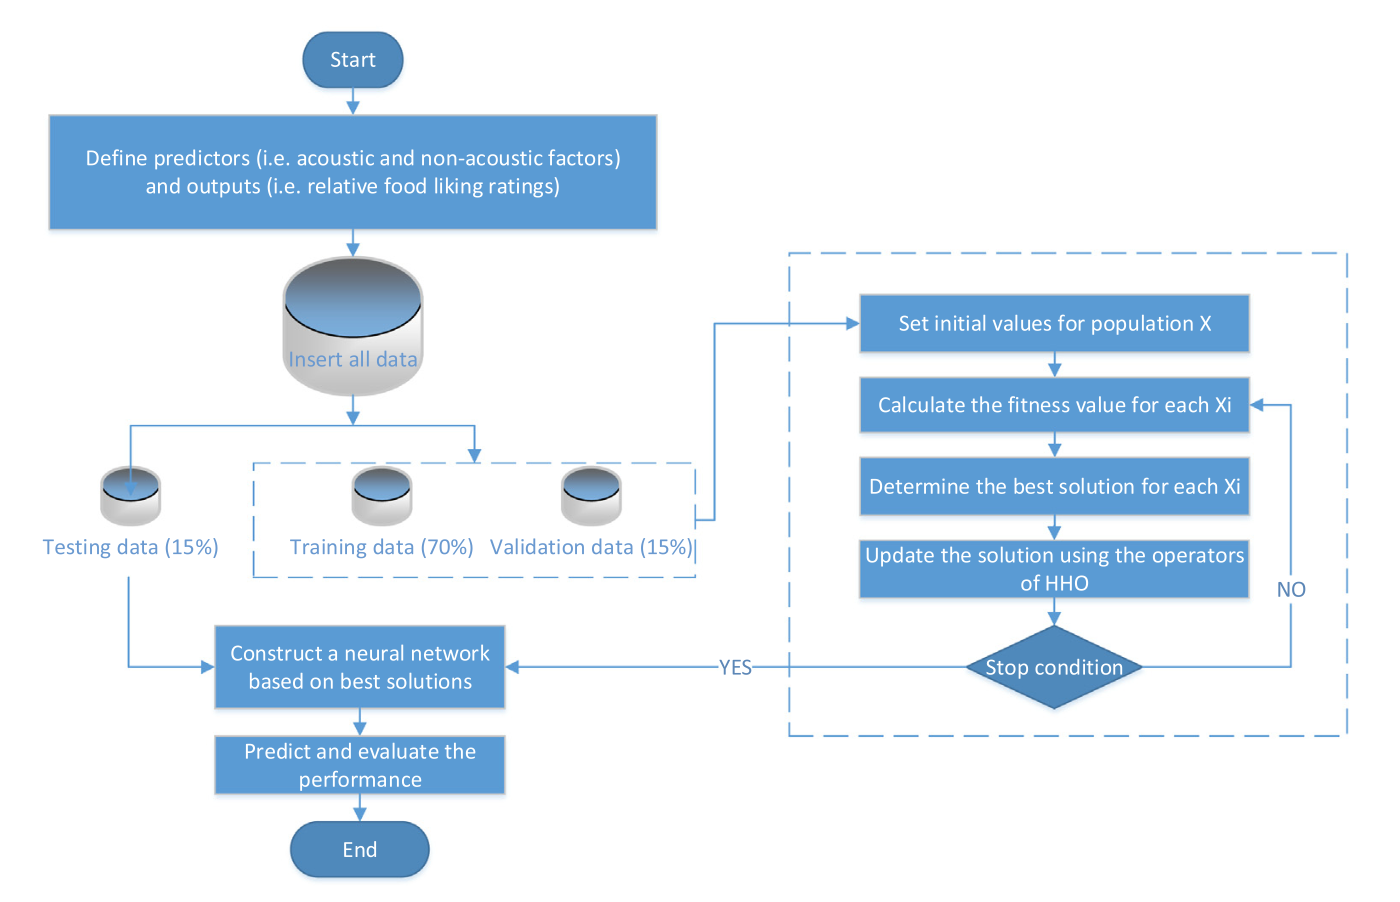
\includegraphics[width=0.9\textwidth]{Chapters/Figures/HHO-ANN.png}
      \caption{Il modello HHO-ANN proposto per la previsione del gradimento del cibo, in relazione al rumore di fondo nell'ambiente di ascolto.}
      \label{hho-ann}
\end{figure}

Grazie alla sua architettura avanzata e all'utilizzo dell'ottimizzazione \gls{hho}, il modello ANN-HHO è risultato altamente efficace nel prevedere la gradevolezza relativa del cibo in presenza di diversi tipi e livelli di rumore di fondo, fornendo uno strumento prezioso per comprendere e mitigare l'impatto acustico nel settore ristorativo.

\subsection{Risultati e analisi delle prestazioni}
\noindent

Questa sezione presenta i risultati del modello ANN-HHO e confronta le sue prestazioni con quelle dei modelli ANN tradizionali e dei modelli statistici misti nella previsione del gradimento dei cibi in presenza di rumore di fondo.

Il confronto delle prestazioni del modello è riportato di seguito:

\begin{itemize}
    \item \textbf{Modello ANN-HHO:}
    \begin{itemize}
        \item R\textsuperscript{2} = 0.70
        \item RMSE = 0.8
        \item MAE = 0.7
    \end{itemize}
    
    \item \textbf{Modello RNA tradizionale (rete neurale feedforward):}
    \begin{itemize}
        \item R\textsuperscript{2} = 0.61
        \item RMSE = 1.1
        \item MAE = 0.8
    \end{itemize}
    
    \item \textbf{Modello statistico misto:}
    \begin{itemize}
        \item R\textsuperscript{2} = 0.42
        \item RMSE = 1.8
        \item MAE = 1.3
    \end{itemize}
\end{itemize}

\begin{figure}[H]
      \centering
      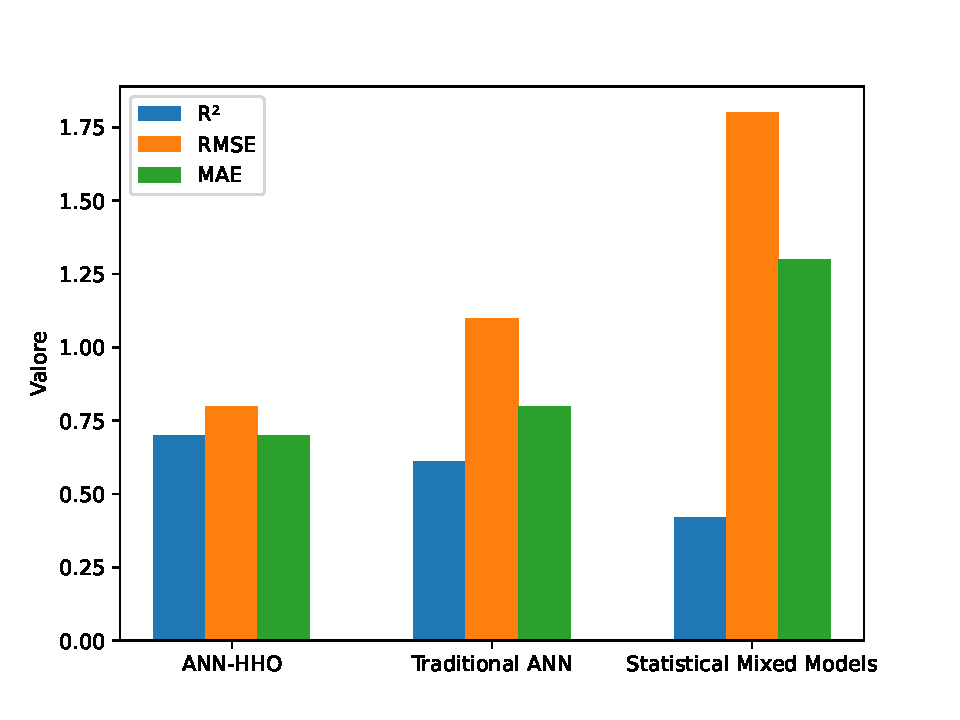
\includegraphics[width=0.7\textwidth]{Chapters/Figures/grafico_performance_modelli.pdf} % Specifica il percorso corretto del tuo file PDF
      \caption{\small Confronto delle prestazioni di ANN-HHO, ANN tradizionale e modelli statistici misti per la previsione del gradimento dei cibi. Il grafico mostra l'R-quadrato (R²), l'errore quadratico medio (RMSE) e l'errore assoluto medio (MAE) per ciascun modello, dimostrando la superiorità delle prestazioni dell'approccio ANN-HHO.}
      \label{fig:graph_label}
\end{figure}

Il modello ANN-HHO dimostra un potere predittivo superiore, spiegando il 70\% della varianza nei giudizi di gradimento dei cibi (R\textsuperscript{2} = 0.70). I valori più bassi di RMSE e MAE indicano che le previsioni del modello ANN-HHO sono più vicine alle valutazioni reali rispetto agli altri modelli. Le prestazioni del modello sul set di test, che comprende il 15\% dei dati, indicano una buona generalizzazione ai dati non visti.

I risultati principali del modello ANN-HHO includono:

\begin{itemize}
    \item \textbf{Livelli ottimali di rumore:} Il modello prevede il massimo gradimento relativo del cibo a livelli di rumore compresi tra 30 e 35 dBA per diversi tipi di rumore.
    
    \item \textbf{Impatto del tipo di rumore:}
    \begin{itemize}
        \item \textit{Musica:} Impatto positivo sul gradimento del cibo fino a 47 dBA.
        \item \textit{Rumore dei ristoranti e del traffico stradale:} Impatto negativo a tutti i livelli studiati.
    \end{itemize}
    
    \item \textbf{Analisi delle soglie:}
    \begin{itemize}
        \item \textit{Musica e rumore del ristorante:} 30 dBA per il massimo gradimento.
        \item \textit{Rumore del traffico stradale:} 35 dBA per il massimo gradimento.
    \end{itemize}
\end{itemize}

\begin{figure}[H]
      \centering
      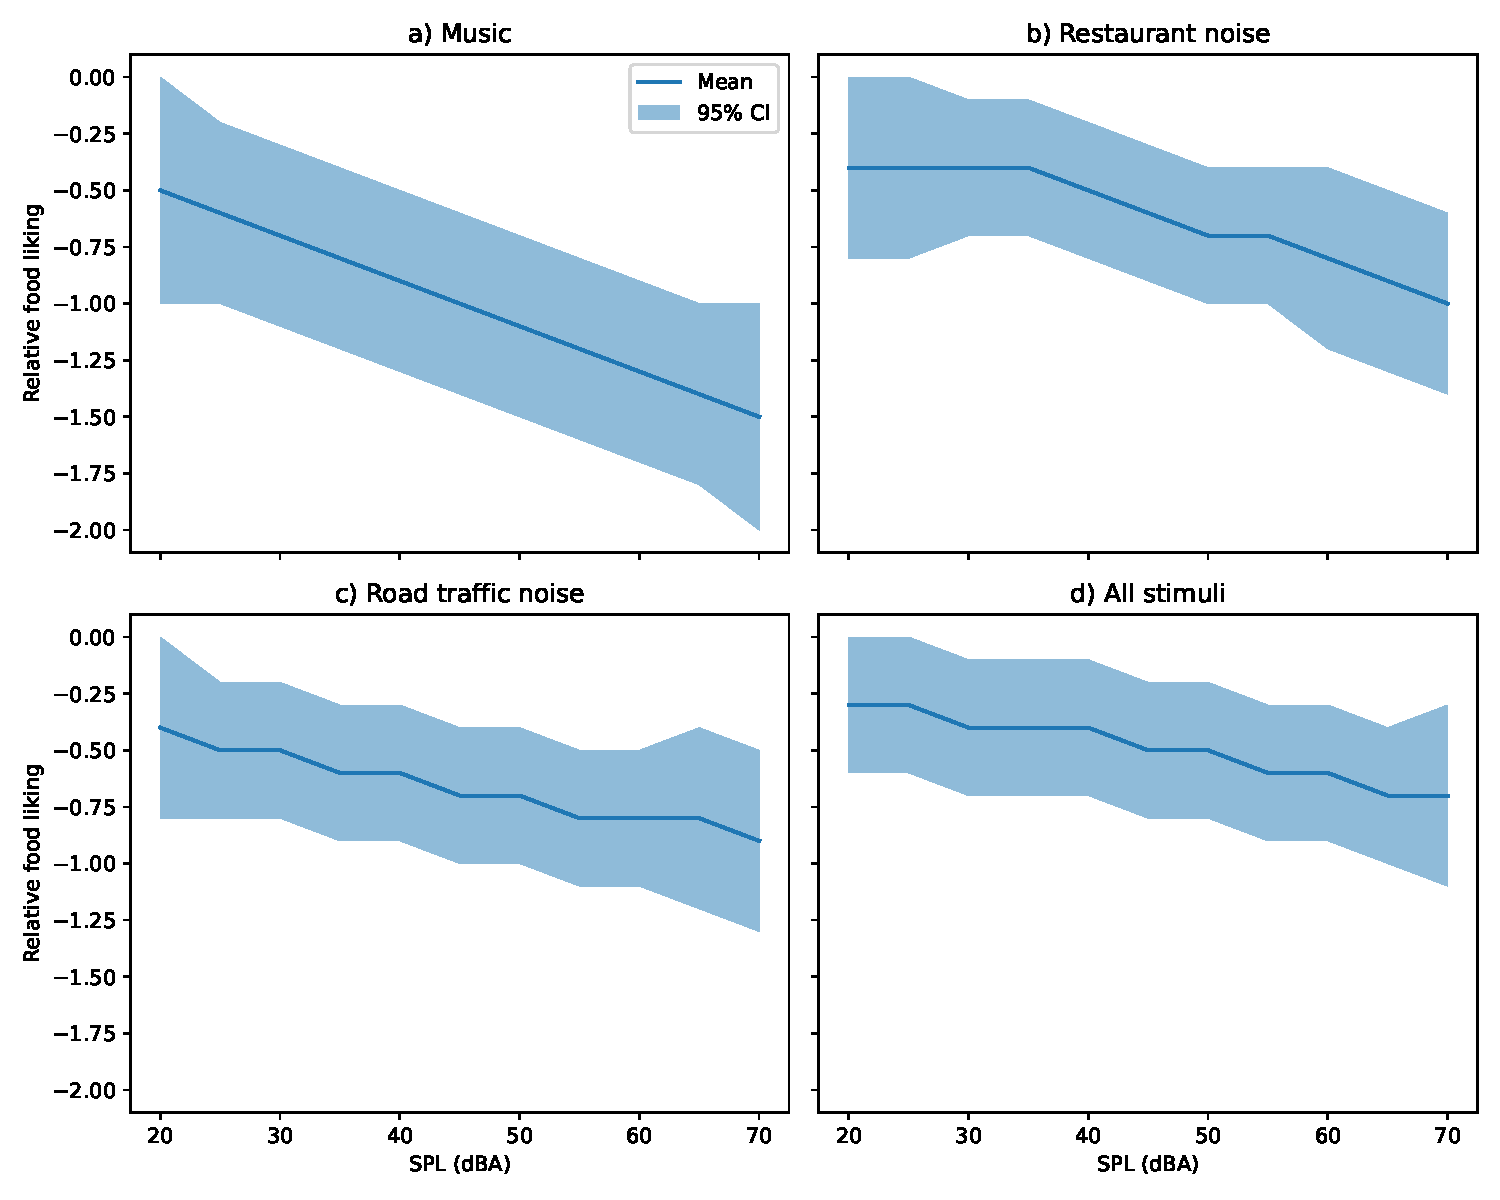
\includegraphics[width=0.7\textwidth]{Chapters/Figures/foodprediction.pdf}
      \caption{\small Previsione del gradimento relativo del cibo a diversi livelli utilizzando la ANN-HHO potenziata per a) musica b) rumore del ristorante c) rumore del traffico stradale e d) tutti gli stimoli acustici. Le linee solide indicano la media e le linee blu ombreggiate indicano le 95{\%} CIs associate alla media.}
      \label{fig:foodprediction}
\end{figure}

Le prestazioni superiori del modello ANN-HHO nella previsione del gradimento del cibo dimostrano il suo potenziale come potente strumento per la comprensione della complessa relazione tra ambiente acustico ed esperienza culinaria. La capacità del modello di identificare i livelli ottimali di rumore e di distinguere tra i vari tipi di rumore offre spunti preziosi sia per i ricercatori che per i professionisti nel campo dell'acustica e della scienza alimentare.

\subsection{Applicazione del modello alla previsione del gradimento del cibo}
\noindent

Questa sezione esplora le implicazioni pratiche e le intuizioni derivate dalle previsioni del modello ANN-HHO per il gradimento del cibo in vari ambienti acustici. \\
\textbf{Ottimizzazione dell'ambiente acustico:} \\
Sulla base delle previsioni del modello, possiamo proporre delle linee guida per un ambiente acustico ottimale nelle aree di ristorazione:
\begin{enumerate}
    \item \textbf{Intervallo di rumore ideale:} Mantenere i livelli di rumore di fondo tra 30-35 dBA per ottimizzare il gradimento del cibo in diversi tipi di rumore.
    \item \textbf{Selezione della musica:} Quando si usa la musica di sottofondo, si possono tollerare livelli fino a 47 dBA senza un impatto negativo significativo sul gradimento del cibo.
    \item \textbf{Attenuazione del rumore:} È necessario prestare particolare attenzione alla riduzione del traffico stradale e del rumore generale dei ristoranti, poiché questi hanno effetti negativi più pronunciati anche a livelli più bassi.
\end{enumerate}

\begin{figure}[H]
      \centering
      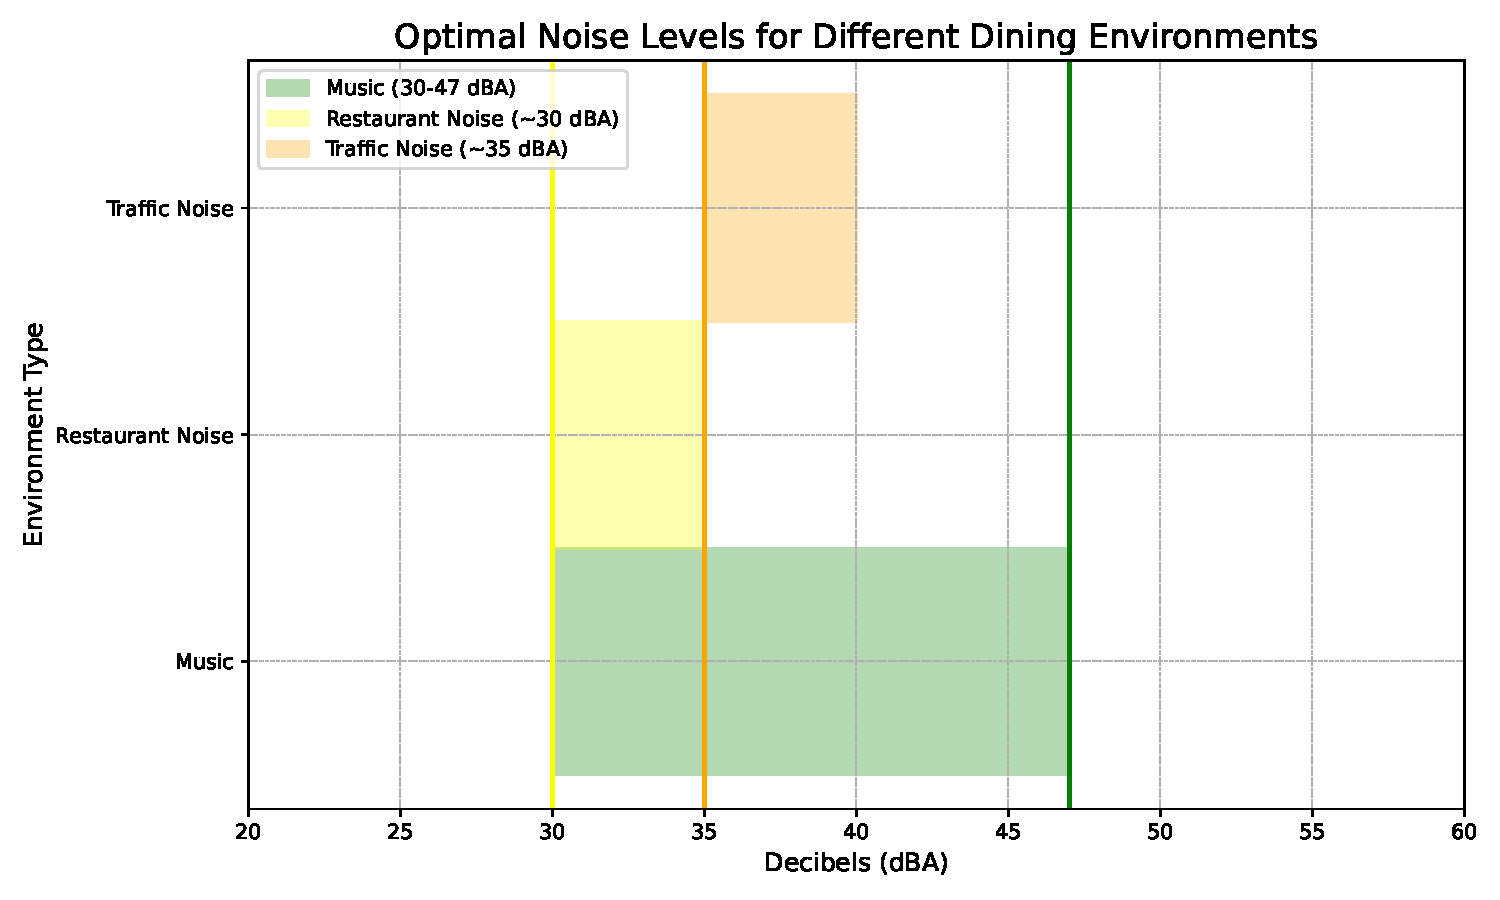
\includegraphics[width=0.7\textwidth]{Chapters/Figures/optimal_noise_levels_improved.pdf} % Specifica il percorso corretto del tuo file PDF
      \caption{\small Livelli di rumorosità ottimali per i diversi ambienti di ristorazione}
      \label{fig:graph_label}
\end{figure}

\textbf{Personalizzazione dell'esperienza culinaria:} \\
La capacità del modello di tenere conto dei fattori individuali consente di fornire raccomandazioni personalizzate:
\begin{enumerate}
    \item \textbf{Considerazioni basate sull'età:} Anche se l'età è risultata essere meno influente, si potrebbero prendere in considerazione dei leggeri aggiustamenti dei livelli di rumore per i diversi gruppi di età.
    \item \textbf{Preferenze specifiche di genere:} Il modello suggerisce lievi variazioni nella tolleranza al rumore tra i due sessi, che potrebbero essere prese in considerazione per la disposizione dei posti a sedere o la suddivisione in zone acustiche dei ristoranti.
    \item \textbf{Adattamento della sensibilità:} Per i clienti con un'elevata sensibilità al rumore, il modello raccomanda un'aderenza più rigorosa all'estremità inferiore dell'intervallo di rumore ottimale.
\end{enumerate}

\textbf{Strategie pratiche di attuazione:}
\begin{enumerate}
    \item \textbf{Zonizzazione acustica:} Progettare i ristoranti con zone acustiche distinte per soddisfare le diverse preferenze e sensibilità.
    \item \textbf{Controllo dinamico del rumore:} Implementare sistemi audio intelligenti che regolano i livelli di rumore in base all'ora del giorno, all'occupazione e ai profili dei clienti.
    \item \textbf{Formazione del personale:} Istruire il personale del ristorante sull'importanza dell'ambiente acustico e su come gestirlo in modo efficace.
\end{enumerate}

% Figure: Conceptual Design of Acoustically Optimized Dining Area [Create a new figure showing a restaurant floor plan with different acoustic zones]%

Queste applicazioni pratiche dimostrano come le intuizioni del modello ANN-HHO possano essere tradotte in strategie attuabili per migliorare le esperienze di ristorazione attraverso l'ottimizzazione dell'ambiente acustico. Considerando sia le tendenze generali sia i fattori individuali, i ristoranti e i locali possono creare atmosfere più piacevoli e personalizzate per i loro clienti.

\subsection{Discussione e implicazioni}
\noindent

Questa sezione esamina le implicazioni dei risultati del modello ANN-HHO, concentrandosi sul loro significato per l'ingegneria informatica e sulle potenziali applicazioni nell'ottimizzazione dell'ambiente acustico.

\textbf{Risultati principali:}
\begin{enumerate}
    \item \textbf{Prestazioni del modello:} 
    \begin{itemize}
        \item RNA-HHO: R² = 0,70, RMSE = 0,8
        \item Ha superato le prestazioni di RNA tradizionali e dei modelli statistici
    \end{itemize}
    \item \textbf{Ambienti acustici ottimali:} 
    \begin{itemize}
        \item Intervallo ottimale generale: 30-35 dBA
        \item Tolleranza della musica fino a 47 dBA
    \end{itemize}
    \item \textbf{Importanza delle caratteristiche:} 
    \begin{itemize}
        \item Fattori acustici (tipo e livello di rumore) più significativi
        \item Fattori non acustici (età, sesso, sensibilità) meno impattanti
    \end{itemize}
\end{enumerate}

\textbf{Implicazioni per l'ingegneria informatica:}
\begin{enumerate}
    \item \textbf{Tecniche avanzate di intelligenza artificiale:} 
    \begin{itemize}
        \item Integrazione riuscita delle reti neurali con l'ottimizzazione ispirata dalla natura
        \item Potenziale per la risoluzione di problemi complessi e multidimensionali
    \end{itemize}
    \item \textbf{Interpretabilità del modello:} 
    \begin{itemize}
        \item L'uso dell'algoritmo “RReliefF” migliora la trasparenza del modello
        \item Affronta i limiti della “scatola nera” delle reti neurali
    \end{itemize}
    \item \textbf{Applicazioni interdisciplinari:} 
    \begin{itemize}
        \item Dimostra la versatilità dell'IA in ambiti non tradizionali
        \item Apre strade per l'IA nella ricerca esperienziale e sensoriale
    \end{itemize}
\end{enumerate}

\textbf{Direzioni di ricerca future:}
\begin{enumerate}
    \item \textbf{Sistemi di previsione in tempo reale:} 
    \begin{itemize}
        \item Sviluppo di modelli dinamici e adattivi
        \item Integrazione con l'IoT per il controllo di ambienti intelligenti
    \end{itemize}
    \item \textbf{Integrazione sensoriale multimodale:} 
    \begin{itemize}
        \item Espansione per includere altri input sensoriali (ad esempio, visivi, olfattivi)
        \item Approccio olistico all'ottimizzazione ambientale
    \end{itemize}
    \item \textbf{Scalabilità e generalizzazione:} 
    \begin{itemize}
        \item Verifica delle prestazioni del modello in diversi contesti
        \item Analisi delle variazioni culturali e geografiche
    \end{itemize}
\end{enumerate}

\begin{figure}[H]
      \centering
      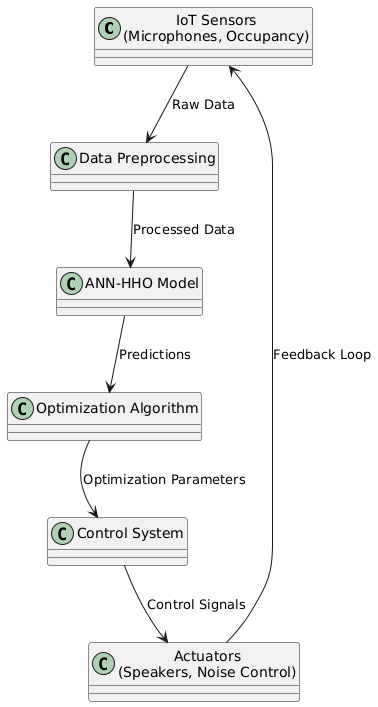
\includegraphics[width=0.4\textwidth]{Chapters/Figures/real_time_system.png}
      \caption{\small Proposed Framework for Real-time Acoustic Optimization System integrating ANN-HHO model.}
      \label{fig:realtimesystem}
\end{figure}

Questa ricerca contribuisce al campo dell'ingegneria informatica dimostrando l'efficacia dei modelli ibridi di intelligenza artificiale nella risoluzione di problemi complessi del mondo reale. Il modello ANN-HHO non solo fornisce previsioni accurate ma offre anche interpretabilità, risolvendo una critica comune alle reti neurali. Il successo dell'applicazione nell'ottimizzazione dell'ambiente acustico apre nuove strade all'IA nella progettazione esperienziale e nella ricerca sensoriale.

I risultati pongono le basi per lo sviluppo di sistemi intelligenti in grado di regolare l'ambiente in tempo reale, rivoluzionando potenzialmente l'approccio alla progettazione acustica degli spazi pubblici. Il lavoro futuro dovrebbe concentrarsi sull'espansione delle capacità del modello, sull'esplorazione di integrazioni multimodali e sullo studio della sua scalabilità in diversi contesti.

\subsection{Limitazioni e lavoro futuro}
\noindent

Questa sezione affronta gli attuali limiti del modello ANN-HHO e delinea le potenziali direzioni di ricerca future per migliorarne le capacità e le applicazioni.

Limitazioni:
\begin{enumerate}
    \item \textbf{Ambito del set di dati:} 
    Limitato a specifici tipi e livelli di rumore. Campione relativamente piccolo (135 risposte).
    \item \textbf{Fattori ambientali:} Si concentra esclusivamente sui fattori acustici, escludendo altri input sensoriali.
    \item \textbf{Diversità culturale:} Potenziale mancanza di validazione interculturale.
    \item \textbf{Applicazione in tempo reale:} Il modello attuale non è ottimizzato per l'elaborazione in tempo reale.
    \item \textbf{Effetti a lungo termine:} Lo studio non tiene conto dell'esposizione prolungata ad ambienti ottimizzati.
\end{enumerate}

Lavoro futuro:
\begin{enumerate}
    \item \textbf{Ampliamento del set di dati:} Incorporare una gamma più ampia di tipi e livelli di rumore. Aumentare la dimensione del campione e la diversità demografica.
    \item \textbf{Integrazione multimodale:} Includere altri fattori sensoriali (ad esempio, illuminazione, temperatura). Sviluppare un modello olistico di ottimizzazione ambientale.
    \item \textbf{Studi interculturali:} Convalidare il modello in diversi contesti culturali. Studiare le variazioni culturali nella percezione del rumore e nel gradimento del cibo.
    \item \textbf{Ottimizzazione in tempo reale:} Sviluppare una versione leggera di ANN-HHO per l'elaborazione in tempo reale. Implementazione e test in ambienti di ristorazione reali.
    \item \textbf{Studi a lungo termine:} Indagare gli effetti degli ambienti acustici ottimizzati per periodi prolungati. Valutare potenziali effetti di assuefazione o sensibilizzazione.
    \item \textbf{Tecniche avanzate di intelligenza artificiale:} Esplorare l'integrazione con altri modelli di IA (ad esempio, l'apprendimento per rinforzo). Studiare l'apprendimento per trasferimento per un rapido adattamento a nuovi ambienti.
    \item \textbf{Personalizzazione:} Sviluppare modelli specifici per ogni individuo per l'ottimizzazione acustica personalizzata. Esplorare le tecniche di tutela della privacy per la gestione dei dati personali.
\end{enumerate}

\begin{figure}[H]
      \centering
      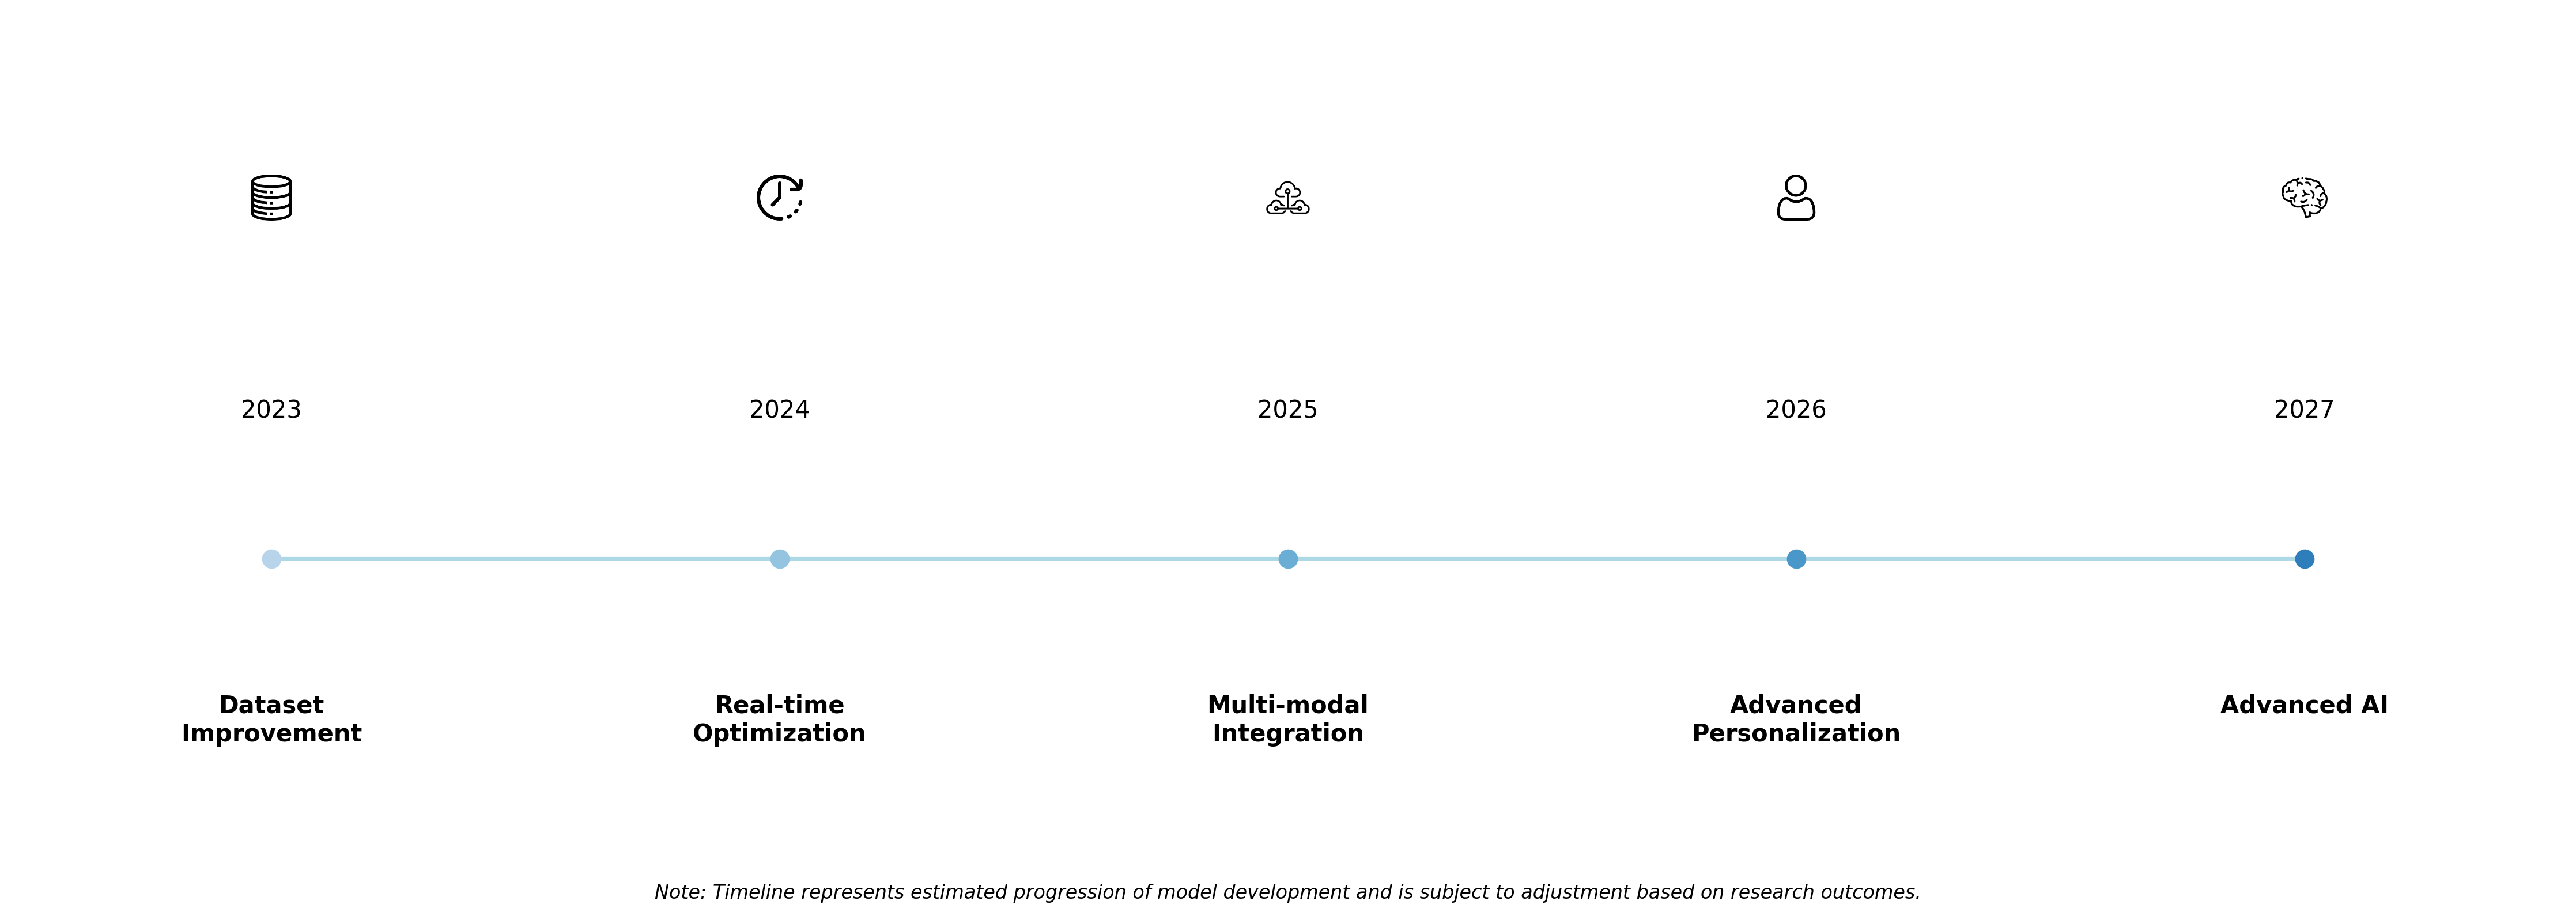
\includegraphics[width=0.9\textwidth]{Chapters/Figures/improved_future_roadmap.png} 
      \caption{\small Proposed Roadmap for Future ANN-HHO Model Development.}
      \label{fig:future_roadmap}
\end{figure}

Affrontando queste limitazioni e perseguendo queste direzioni di ricerca future, possiamo migliorare significativamente le capacità del modello ANN-HHO e ampliarne l'applicabilità. La tabella di marcia proposta mira a far evolvere il modello attuale in uno strumento più robusto, versatile e praticamente applicabile per l'ottimizzazione dell'ambiente acustico.

L'integrazione di dati sensoriali multimodali e lo sviluppo di capacità di elaborazione in tempo reale rappresentano strade particolarmente promettenti per il lavoro futuro. Questi progressi potrebbero portare alla creazione di sistemi intelligenti in grado di ottimizzare dinamicamente ambienti complessi, con applicazioni potenziali che vanno ben oltre il contesto iniziale delle esperienze gastronomiche.